In \secref{prior_perturbations} we considered a multiplicative perturbations
of the form \eqref{phi_perturbation} with the $\norminf{\cdot}$ norm.  In
this section we consider other norms, illustrating that other choices
have problems with KL divergence.

We begin with an example from \citet{averbukh:1967:theory}.

%%%%%%%%%%%%%%%%%%%%%%%%%%%%%%%%%%%%%%%%%%%%%%%%%%%%%%%%%%%%%%%%%%%%%%%%%
%%%%%%%%%%%%%%%%%%%%%%%%%%%%%%%%%%%%%%%%%%%%%%%%%%%%%%%%%%%%%%%%%%%%%%%%%
\begin{ex}\exlabel{averbukh}
%
(\citet[Example 1.9]{averbukh:1967:theory})
%
Consider $(x_1, x_2) \in \mathbb{R}^2$ and the polar coordinates $r :=
\sqrt{x_1^2 + x_2^2}$ and $\theta := \arctan(x_2 / x_1)$.  Let $\{\pi k: k \in
\mathbb{Z} \}$ denote integer multiples of $\pi$.  Define
%
\begin{align*}
%
f(r, \theta) := \begin{cases}
\frac{r^2}{| \sin \theta |} \exp\left( -\frac{r}{|\sin \theta|}\right)
    & \textrm{when } \theta \notin \{\pi k: k \in \mathbb{Z} \} \\
0. & \textrm{when } \theta \in \{\pi k: k \in \mathbb{Z} \}
%
\end{cases}
%
\end{align*}
%
Then $f$ is continuous at $(0, 0)$ and has a directional derivative in every
direction, but is not Fr{'e}chet differentiable.
%
\end{ex}
%%%%%%%%%%%%%%%%%%%%%%%%%%%%%%%%%%%%%%%%%%%%%%%%%%%%%%%%%%%%%%%%%%%%%%%%%
%
See \figref{averbukh}.
%
%%%%%%%%%%%%%%%%%%%%%%%%%%%%%%%%%%%%%%%%%%%%%%%%%%%%%%%%%%%%%%%%%%%%%%%%%
%%%%%%%%%%%%%%%%%%%%%%%%%%%%%%%%%%%%%%%%%%%%%%%%%%%%%%%%%%%%%%%%%%%%%%%%%
\begin{figure}[h!]\figlabel{averbukh}
\caption{A plot of $f(x_1, x_2)$ from \exref{averbukh}.}

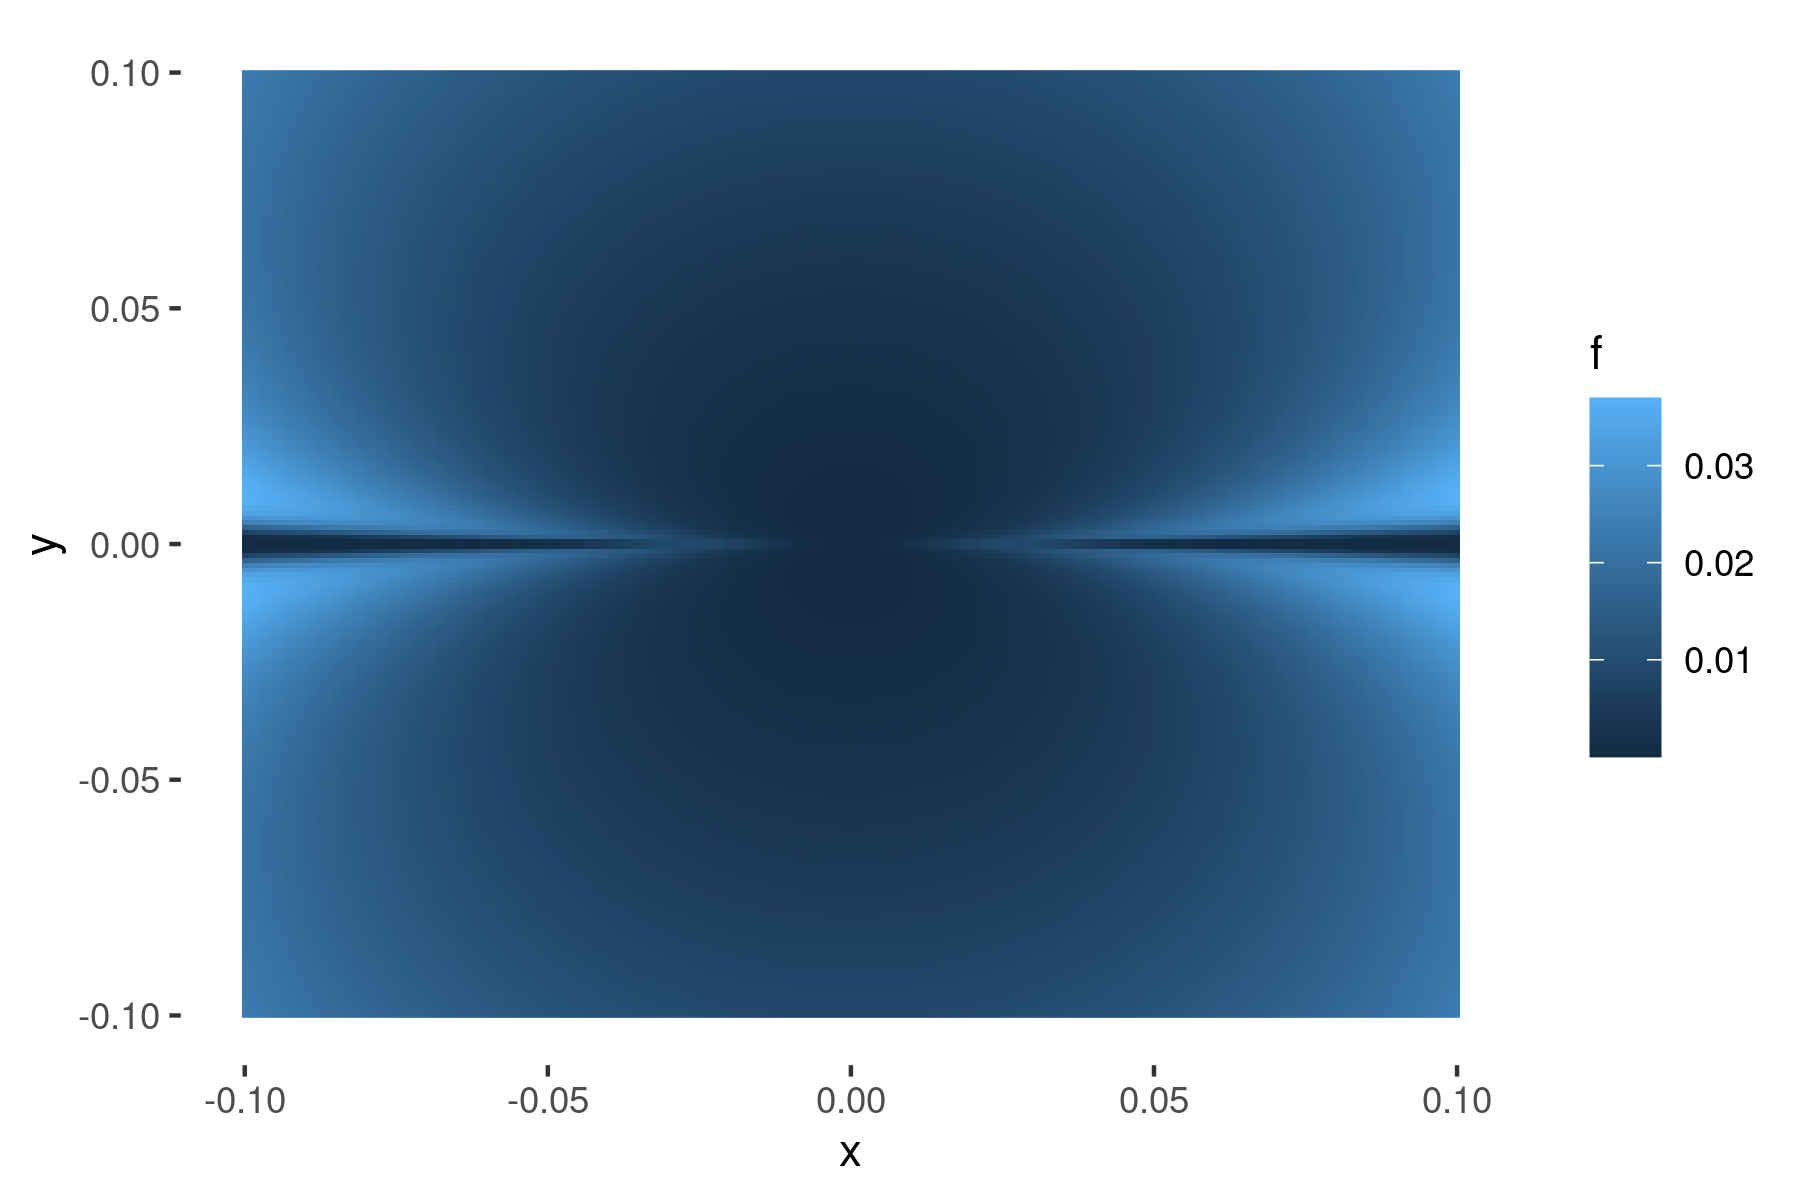
\includegraphics[width=0.980\linewidth,height=0.667\linewidth]{static_images/averbukh_example.png}
\centering
\end{figure}
%%%%%%%%%%%%%%%%%%%%%%%%%%%%%%%%%%%%%%%%%%%%%%%%%%%%%%%%%%%%%%%%%%%%%%%%%
